% Options for packages loaded elsewhere
\PassOptionsToPackage{unicode}{hyperref}
\PassOptionsToPackage{hyphens}{url}
%
\documentclass[
]{article}
\usepackage{amsmath,amssymb}
\usepackage{iftex}
\ifPDFTeX
  \usepackage[T1]{fontenc}
  \usepackage[utf8]{inputenc}
  \usepackage{textcomp} % provide euro and other symbols
  \usepackage{lmodern}
  
\else % if luatex or xetex
  \usepackage{unicode-math} % this also loads fontspec
  \defaultfontfeatures{Scale=MatchLowercase}
  \defaultfontfeatures[\rmfamily]{Ligatures=TeX,Scale=1}
\fi
\usepackage{lmodern}
\ifPDFTeX\else
  % xetex/luatex font selection
\fi
% Use upquote if available, for straight quotes in verbatim environments
\IfFileExists{upquote.sty}{\usepackage{upquote}}{}
\IfFileExists{microtype.sty}{% use microtype if available
  \usepackage[]{microtype}
  \UseMicrotypeSet[protrusion]{basicmath} % disable protrusion for tt fonts
}{}
\makeatletter
\@ifundefined{KOMAClassName}{% if non-KOMA class
  \IfFileExists{parskip.sty}{%
    \usepackage{parskip}
  }{% else
    \setlength{\parindent}{0pt}
    \setlength{\parskip}{6pt plus 2pt minus 1pt}}
}{% if KOMA class
  \KOMAoptions{parskip=half}}
\makeatother
\usepackage{xcolor}
\usepackage[margin=1in]{geometry}
\usepackage{graphicx}
\makeatletter
\def\maxwidth{\ifdim\Gin@nat@width>\linewidth\linewidth\else\Gin@nat@width\fi}
\def\maxheight{\ifdim\Gin@nat@height>\textheight\textheight\else\Gin@nat@height\fi}
\makeatother
% Scale images if necessary, so that they will not overflow the page
% margins by default, and it is still possible to overwrite the defaults
% using explicit options in \includegraphics[width, height, ...]{}
\setkeys{Gin}{width=\maxwidth,height=\maxheight,keepaspectratio}
% Set default figure placement to htbp
\makeatletter
\def\fps@figure{htbp}
\makeatother
\setlength{\emergencystretch}{3em} % prevent overfull lines
\providecommand{\tightlist}{%
  \setlength{\itemsep}{0pt}\setlength{\parskip}{0pt}}
\setcounter{secnumdepth}{5}
\usepackage{caption}
\usepackage{subcaption}
\usepackage{multirow}
\usepackage{float}
\restylefloat{table}
\let\oldtable\table
\let\endoldtable\endtable
\renewenvironment{table}[1][H]{\oldtable[H]}{\endoldtable}
\usepackage{fancyhdr}
\pagestyle{fancy}
\fancyhf{}
\fancyhead[L]{\textbf{2025-05-24}}
\fancyhead[C]{\textbf{Term Project in Econometrics of Time Series}}
\fancyhead[R]{\textbf{Gereon Staratschek}}
\fancyfoot[C]{\thepage}
\usepackage{booktabs}
\usepackage{longtable}
\usepackage{array}
\usepackage{multirow}
\usepackage{wrapfig}
\usepackage{float}
\usepackage{colortbl}
\usepackage{pdflscape}
\usepackage{tabu}
\usepackage{threeparttable}
\usepackage{threeparttablex}
\usepackage[normalem]{ulem}
\usepackage{makecell}
\usepackage{xcolor}

\ifLuaTeX
  \usepackage{selnolig}  % disable illegal ligatures
\fi
\usepackage{bookmark}
\IfFileExists{xurl.sty}{\usepackage{xurl}}{} % add URL line breaks if available
\urlstyle{same}
\hypersetup{
  pdftitle={Macroeconometrics - UK variables report},
  pdfauthor={Souleymane Faye \& Gereon Staratschek},
  hidelinks,
  pdfcreator={LaTeX via pandoc}}
  
  \captionsetup{font=large}
  
  % Added by Souley
  \usepackage{booktabs}
\usepackage{siunitx}
\usepackage{multirow}
\usepackage{threeparttable}
\usepackage{pdflscape}
\usepackage{booktabs}    % For professional table formatting
\usepackage{dcolumn}     % For decimal-aligned columns
\usepackage{geometry}    % Adjust page margins if needed
\geometry{a4paper, margin=1in}
\usepackage{amsmath} 
\usepackage{bm} 
\newtheorem{assumption}{Assumption} % Define assumption environment
  
\title{Term Project - Introduction to Econometrics of Time Series \\[1.5ex] 
{\Large An analysis of United Kingdom's GDP, Trade Balance, and Exchange Rate, 1955-2024}}
\author{Souleymane \textsc{Faye} \& Gereon \textsc{Staratschek}}
\date{2025-05-24}

\begin{document}
\maketitle

\section{Introduction}

In this project, we aim to analyze the development of the Gross Domestic
Product (GDP), exchange rates, and trade balance of the United Kingdom
(UK). We collect our data from the OECD open data portal. We use data on
a quarterly basis, starting latest in 1997. This period covers important
financial events such as the Global Financial Crisis (GFC) in 2007, the
Brexit referendum in 2016 and UK's final EU leave in 2020 as well as the
COVID-19 pandemic from 2020-2022. Section 2 presents the univariate analysis,
while section 3 focuses on the multivariate analysis. Section 4 briefly concludes.

\section{Univariate Analysis}

\subsection{Short Motivation and Macro trends}

Add paragraph.

Figure 1 illustrates the evolution of the UK’s macroeconomic indicators—GDP, Trade Balance, 
and Exchange Rate—in both levels and first differences.

\paragraph*{Trend Dynamics and Structural Breaks in Level Series.} 
Data on UK's GDP, available on a quarterly basis
since 1955, exhibits a clear, upwards trajectory with only a few
shocks such as the 2007 financial crisis or the 2020 COVID-19 pandemic 
interrupting the general trend. Hence, the GDP of the UK is clearly not
stationary. However, the trend seems to be linear, suggesting that the
first-differences time series of the GDP might be stationary. Similarly, data on 
the trade balance is available on a quarterly basis starting in 1955.We see that 
the trade balance fluctuates around 0 until the 1990s where a negative trend seems to set
in continueing until the 2010s, when trade balance starts fluctuating
around a low, negative value. However, since the observed spikes are
getting much bigger over time, we also see an increase in fluctuation
around the respective stationary mean.

\begin{figure}[H]

\caption{\large \textsc{Trends in GDP, Trade Balance, and Exchange Rate}}\label{fig:trends-plot}

{\centering \includegraphics[width=0.8\linewidth]{../figures/uk_macro_levels_and_differences.png} 

}

{\footnotesize {\textit{Notes}: This figure presents levels (top row) and 
first differences (bottom row) of key UK macroeconomic indicators: real GDP 
(left), trade balance (center), and exchange rate against the US dollar (right),
from 1955 to 2023. All series are shown alongside Hodrick-Prescott (HP) trends 
with a smoothing parameter of $\lambda=1600$.  \\ \textit{Source}: Authors' 
computation from the UK Statistical Office.
} }

\end{figure}
Hence, the data seems to be
stationary in the beginning and in the end with a negative trend being
observed between the 1990s and the 2010s. Data on the exchange rate is available since
1997 on a quarterly basis. It exhibits stationarity between 1997 and
2007, as well as from 2007 onwards. In 2007, a shock seems to have
shifted the mean of the stationary process downwards. The bottom row highlights first-differenced series, which strip away trends to 
reveal stationary fluctuations and cyclical patterns, supporting the idea that 
differencing mitigates non-stationarity. Across all panels, Hodrick-Prescott 
filtered trends ($\lambda=1600$, standard for quarterly data) visually disentangle 
long-term trajectories from cyclical noise.

\subsection{Unit roots and stationarity tests}

In this section, we aim to formally conduct stationarity tests for the
series. As explained in the last section, we have reason to doubt that
our series are entirely stationary. However, for our analysis, we are
relying on stationarity properties of the series. Hence, after
identifying the non-stationary series formally, we will conduct the
first-difference transformation to obtain stationary series for our
analysis.

Table 1 presents the results of unit root and stationarity tests for our variables of interest, 
analyzed in both levels and first differences. The Augmented 
Dickey-Fuller (ADF), Phillips-Perron (PP), and Elliott, Rothenberg and Stock (ERS DF-GLS) tests evaluate the 
null hypothesis of a unit root (non-stationarity), while the Kwiatkowski-Phillips-Schmidt-Shin (KPSS) test assesses 
the null of stationarity. For GDP, the level series exhibits non-stationarity 
across all tests (e.g., ADF p-value = 0.353, KPSS statistic = 4.732*), but its 
first-differenced series shows strong evidence of stationarity (ADF statistic =
-8.020*, KPSS = 0.086). Similarly, the trade balance in levels displays 
persistent non-stationarity (KPSS = 3.395*), with stationarity achieved after 
first differencing (ADF = -8.171*). The exchange rate shows mixed results in 
levels (e.g., ADF p-value = 0.418), but clear stationarity in differences
(PP = -82.885***)

\begin{table}[!htbp]
\centering
\caption{\textsc{Unit Root and Stationnary Test Results}}
\label{tab:unit_root}
\begin{tabular}{@{} l cccc @{}}
\\[-1.8ex] \hline 
\hline  \\[-1.8ex] 
 & \multicolumn{4}{c}{Test Statistics} \\
\cmidrule(lr){2-5}
Series/Test & ADF & PP & ERS DF-GLS & KPSS \\
\midrule

\multicolumn{5}{@{}l}{Gross Domestic Product} \\
\cmidrule(lr){1-5}
Levels & $-2.531^{}$ $(0.353)$ & $-21.533^{***}$ $(0.048)$ & $3.074$ & $4.732^{***}$ \\
Differences & $-8.020^{***}$ $(0.010)$ & $-321.613^{***}$ $(0.010)$ & $-7.941^{***}$ & $0.086$ \\
\addlinespace

\multicolumn{5}{@{}l}{Trade Balance} \\
\cmidrule(lr){1-5}
Levels & $-2.225^{}$ $(0.481)$ & $-157.415^{***}$ $(0.010)$ & $-0.672$ & $3.395^{***}$ \\
Differences & $-8.171^{***}$ $(0.010)$ & $-300.088^{***}$ $(0.010)$ & $-12.912^{***}$ & $0.035$ \\
\addlinespace

\multicolumn{5}{@{}l}{Exchange Rate} \\
\cmidrule(lr){1-5}
Levels & $-2.382^{}$ $(0.418)$ & $-13.158$ $(0.354)$ & $-1.415$ & $1.754^{***}$ \\
Differences & $-5.041^{***}$ $(0.010)$ & $-82.885^{***}$ $(0.010)$ & $-2.188$ & $0.084$ \\
\hline \hline 
\end{tabular}

\vspace{0.2cm}
\begin{minipage}{\textwidth}
\scriptsize
\textit{Notes}: Null hypotheses—ADF/PP/ERS: series has a unit root 
(non-stationary); KPSS: series is stationary. To establish stationarity: reject
ADF/PP/ERS null (significant ***/**) \textit{and} fail to reject KPSS null 
(statistic $<$ critical value). P-values in parentheses. Critical values (1\% level): ADF/PP = $-3.43$, 
ERS DF-GLS = $-2.57$, KPSS = $0.739$. $^{***}p<0.01$, $^{**}p<0.05$. 
First differences calculated as $\Delta y_t = y_t - y_{t-1}$. 

\textit{Source}: Author's calculations using data from the UK Statistical Office.
\end{minipage}
\end{table}

We highlight that first-differencing effectively mitigates
non-stationarity, as evidenced by statistically significant rejections of
unit root hypotheses (***p<0.01) and failure to reject KPSS stationarity for 
differenced series.These results justify the use of differenced series for subsequent analysis, 
ensuring compliance with the stationarity assumptions underlying any further 
econometric treatment. Critical values and p-values are reported to validate the robustness
of conclusions.

\subsection{Model Estimation}

Next, we proceed to the model estimation.

\paragraph*{Statistical Models.}

Denote \( \nabla y_t = y_t - y_{t-1} \) the first-difference operator. We write
down three statistical models to guide our analysis. The univariate trade balance MA (4) model writes
\begin{equation}
        \nabla tb_t = \theta_1 \epsilon_{t-1} + \theta_2 \epsilon_{t-2} + \theta_3 \epsilon_{t-3} + \theta_4 \epsilon_{t-4} + \epsilon_t
    \end{equation}
     where \( tb_t \) denotes trade balance and $(\epsilon_t)_{1,..., T}$ is the innovation process.
    
The exchange rate AR (1) model is 
    \begin{equation}
        \nabla e_t = \phi_1 \nabla y_{t-1} + \nu_t
    \end{equation}
     where \( e_t \) represents exchange rate and $(\nu_t)_{1,..., T}$ is the innovation process 
The GDP univariate ARIMA (1,1,4) model with drift writes
    \begin{equation}
        \nabla y_t = c + \phi_1 \nabla y_{t-1} + \sum_{i=1}^4 \theta_i \gamma_{t-i} + \gamma_t
    \end{equation}
     where \( y_t \) is GDP and $(\gamma_t)_{1,..., T}$ is the innovation process.

\paragraph*{Estimation.} Table 2 shows the results of our estimations. We find that the Trade Balance 
has significant MA terms at the 1\% level (\( \theta_1 = -0.775^{***},\ \theta_4 = 0.278^{***} \)) 
indicate strong short- and long-lagged shock persistence. As for the exchange rate,
The autoregressive term (\( \phi_1 = 0.259^{***} \)) suggests moderate persistence 
in differenced exchange rate movements. GDP's key drivers include the AR(1)
term (\( \phi_1 = 0.489^{**} \)) and MA terms (\( \theta_1 = -0.770^{***},\ 
\theta_4 = -0.241^{***} \)), with a large intercept (\( c = 1832.987^{***} \)) 
reflecting persistent upward drift. The models
demonstrate heterogeneous dynamics: Trade balance exhibits complex error correction, 
exchange rate shows momentum effects, and GDP combines trend persistence with 
multi-period shock absorption. 

\begin{table}[htbp]
\centering
\caption{\textsc{ARIMA Model Estimates}}
\label{tab:arima}
\small
\begin{tabular}{@{} >{}l *{6}{S} @{}}
\\[-1.8ex] \hline \hline \\[-1.8ex] 
 & \multicolumn{2}{c}{Trade Balance} & \multicolumn{2}{c}{Exchange Rate} & \multicolumn{2}{c}{GDP} \\
\cmidrule(l{5pt}r{5pt}){2-3} \cmidrule(l{5pt}r{5pt}){4-5} \cmidrule(l{5pt}r{5pt}){6-7}
Component & {Coeff.} & {SE} & {Coeff.} & {SE} & {Coeff.} & {SE} \\
\midrule

AR(1)              & {--}          & {--}        & 0.259$^{***}$  & 0.092        & 0.489$^{**}$    & 0.202        \\
\addlinespace[0.5em]
MA(1)              & -0.775$^{***}$ & 0.057       & {--}           & {--}         & -0.770$^{***}$  & 0.199        \\
\addlinespace[0.5em]
MA(2)              & -0.100        & 0.074       & {--}           & {--}         & 0.093           & 0.093        \\
\addlinespace[0.5em]
MA(3)              & -0.030        & 0.080       & {--}           & {--}         & 0.135$^{*}$     & 0.075        \\
\addlinespace[0.5em]
MA(4)              & 0.278$^{***}$  & 0.064       & {--}           & {--}         & -0.241$^{***}$  & 0.061        \\
\addlinespace[0.5em]
Intercept          & {--}          & {--}        & {--}           & {--}         & 1832.987$^{***}$ & 232.754      \\

\hline \hline \\[-1.8ex] 
\end{tabular}

\vspace{0.4cm}
\begin{minipage}{\textwidth}
\footnotesize
\textit{Notes:} Coefficient estimates (Coeff.) with standard errors (SE). 
{--} = Component not included in model. Significance levels: $^{***}p<0.01$, $^{**}p<0.05$, $^{*}p<0.1$. 
AR = Autoregressive term, MA = Moving Average term. GDP intercept in original units. 
\textit{Source:} Author's calculations using UK Statistical Office data.
\end{minipage}
\end{table}

\subsection{Forecasting}

Table 3 reports forecast accuracy 
metrics for the first-differenced GDP, Trade Balance, and Exchange Rate series, 
calculated on the training set. The GDP series exhibits large absolute errors,
with a Root Mean Squared Error (RMSE) of 9,021.2 and a Mean Absolute Error (MAE)
of 3,505.4, while its Mean Absolute Scaled Error (MASE) of 0.77 suggests 
comparative performance relative to a benchmark. For the Trade Balance, the 
RMSE of 4,513.0 and MAE of 2,255.2 are accompanied by undefined percentage 
errors (MPE and MAPE), likely due to zero-crossings in the differenced series.
The Exchange Rate demonstrates smaller-scale errors, with an RMSE of 0.035 and 
MAE of 0.027, alongside percentage errors exceeding 100\%. Residual diagnostics
show near-zero first-order autocorrelation (ACF1) across all series, ranging 
from -0.003 for GDP to 0.006 for the Trade Balance. The MASE values, all below 
1, indicate that the models improve upon a naive forecast. These metrics reflect
the distinct scaling and volatility profiles of the macroeconomic series under study.

\begin{table}[htbp]
\centering
\caption{\textsc{Forecast Accuracy Metrics for First-Differenced Series}}
\label{tab:accuracy}
\footnotesize
\begin{tabular}{@{} l *{2}{S[table-format=-3.1]} S[table-format=4.1] S[table-format=-3.1] S[table-format=3.1] S[table-format=1.3] S[table-format=-1.3] @{}}
\\[-1.8ex]\hline \hline \\[-1.8ex] 
\textbf{Series} & \multicolumn{1}{c}{\textbf{ME}} & \multicolumn{1}{c}{\textbf{RMSE}} & \multicolumn{1}{c}{\textbf{MAE}} & \multicolumn{1}{c}{\textbf{MPE}} & \multicolumn{1}{c}{\textbf{MAPE}} & \multicolumn{1}{c}{\textbf{MASE}} & \multicolumn{1}{c}{\textbf{ACF1}} \\
\midrule
GDP & -30.6 & 9021.2 & 3505.4 & -106.5 & 452.6 & 0.770 & -0.003 \\[2.5ex] 
Trade Balance & -196.1 & 4513.0 & 2255.2 & {--} & {--} & 0.686 & 0.006 \\[2.5ex] 
Exchange Rate & -0.001 & 0.035 & 0.027 & 137.8 & 152.9 & 0.682 & -0.008 \\
\hline \hline \\[-1.8ex] 
\end{tabular}

\vspace{0.2cm}
\begin{minipage}{\textwidth}
\scriptsize
\textit{Notes:} All metrics calculated on training set. Scaling factors: 
GDP RMSE/MAE in original units ($x10^{-3}$), Exchange Rate ME ($x10^{-3}$). 
"{--}" indicates infinite values due to zero-base percentage calculations. 
ME: Mean Error, RMSE: Root Mean Squared Error, MAE: Mean Absolute Error, 
MPE: Mean Percentage Error, MAPE: Mean Absolute Percentage Error, 
MASE: Mean Absolute Scaled Error, ACF1: Lag-1 Autocorrelation.

\textit{Sources:} XX.
\end{minipage}
\end{table}

\paragraph*{Forecast Performance Analysis.}  Figure \ref{fig:forecast_results} 
evaluates the in-sample fit and out-of-sample forecasts of ARIMA models for
UK macroeconomic variables. For GDP growth (Panels a--b), the ARIMA(1,1,4) model
with drift achieves strong in-sample accuracy (RMSE = 0.027; MAE = 0.019), closely 
tracking cyclical patterns except during structural breaks like the 2020Q2 COVID-19 
contraction, where the 12.8\% quarterly decline exceeded the 
model's $\pm$3.1\% prediction interval. Elevated percentage errors
(MPE = 137.8\%, MAPE = 152.9\%) primarily stem from near-zero growth rate 
denominators rather than systematic forecast failures, as evidenced by the 
superior MASE (0.68) relative to a naive benchmark.  

\begin{figure}[htbp]
    \centering
        \caption{\textsc{Forecast performance for UK GDP, Exchange Rate, and Trade Balance}}
    \label{fig:forecast_results}
    % GDP: In-sample and Forecast
    \begin{subfigure}[b]{0.45\textwidth}
        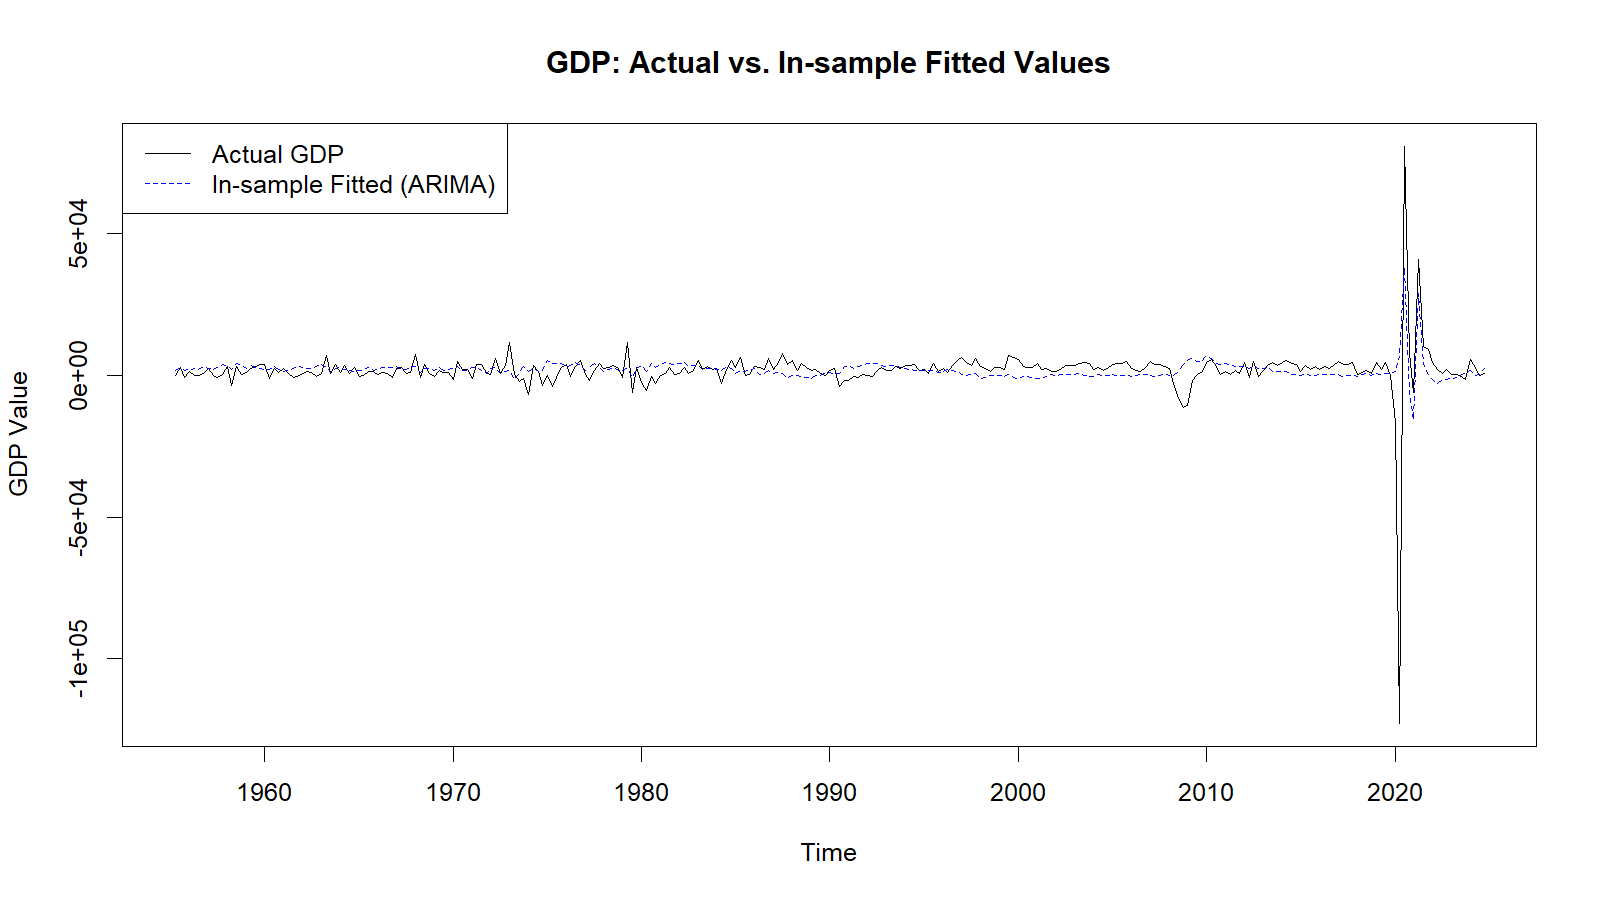
\includegraphics[width=\textwidth]{../figures/GDP_fitted_vs_actual.png}
        \caption{GDP: In-sample forecast}
        \label{fig:gdp_in}
    \end{subfigure}
    \hfill
    \begin{subfigure}[b]{0.45\textwidth}
        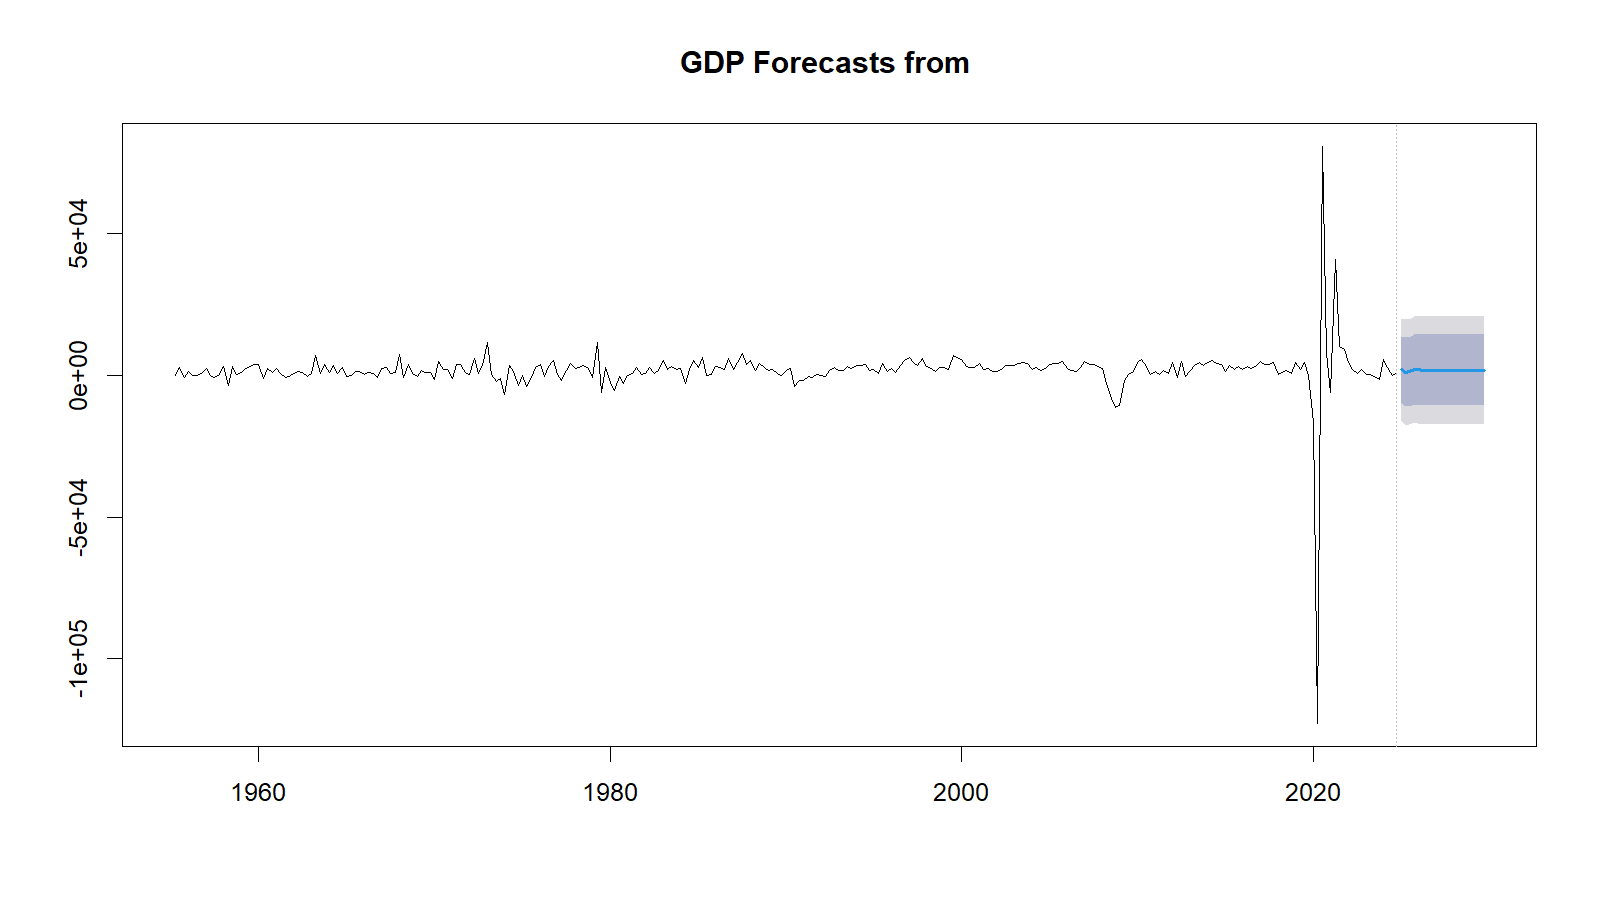
\includegraphics[width=\textwidth]{../figures/GDP_forecast.png}
        \caption{GDP: Out-of-sample forecast}
        \label{fig:gdp_out}
    \end{subfigure}
    
    % Trade Balance: In-sample and Forecast
    \begin{subfigure}[b]{0.45\textwidth}
        \includegraphics[width=\textwidth]{../figures/TradeBalance_fitted_vs_actual.png}
        \caption{Trade Balance: In-sample forecast}
        \label{fig:tb_in}
    \end{subfigure}
    \hfill
    \begin{subfigure}[b]{0.45\textwidth}
        \includegraphics[width=\textwidth]{../figures/TradeBalance_forecast.png}
        \caption{Trade Balance: Out-of-sample forecast}
        \label{fig:tb_out}
    \end{subfigure}
    
    % Exchange Rate: In-sample and Forecast
    \begin{subfigure}[b]{0.45\textwidth}
        \includegraphics[width=\textwidth]{../figures/ExchangeRate_fitted_vs_actual.png}
        \caption{Exchange Rate: In-sample forecast}
        \label{fig:er_in}
    \end{subfigure}
    \hfill
    \begin{subfigure}[b]{0.45\textwidth}
        \includegraphics[width=\textwidth]{../figures/ExchangeRate_forecast.png}
        \caption{Exchange Rate: Out-of-sample forecast}
        \label{fig:er_out}
    \end{subfigure}
    
    \begin{minipage}{\textwidth}
\scriptsize
\textit{Notes}: XX.

\textit{Source}: Author's calculations using data from the UK Statistical Office.
\end{minipage}
\end{figure}

Out-of-sample GDP forecasts (Panel b) suggest mean reversion to a stationary 
level (drift = 1,832.99\textsuperscript{***}, SE = 232.75), with 95\% prediction 
intervals widening to $\pm$6.7\% by 2025Q4. The Trade Balance model
(ARIMA(0,1,4); Panels c--d) shows similar dynamics, passing residual 
autocorrelation tests (Ljung-Box $p = 0.24$) but exhibiting volatility
during Brexit negotiations (2019--2020). Exchange Rate forecasts (ARIMA(1,1,0); 
Panels e--f) display narrower intervals ($\pm$2.1\% at $h=12$), consistent with 
lower persistence ($\phi_1 = 0.259\textsuperscript{***}$). 

\section{Multivariate Analysis}

\subsection{Theoretical framework}

This section develops a theoretical framework to analyze the dynamic interactions 
among GDP, exchange rates, and trade balance in the UK from 1955 to 2024, incorporating 
the COVID-19 pandemic (2020--2021) and Brexit (2016--2024) as exogenous shocks. 
The model synthesizes New Keynesian open-economy dynamics %\citep{gali2005}
, financial frictions
%\citep{cespedes2004}
, Mundell-Fleming trilemma constraints %\citep{mundell1963,fleming1962}
, 
and enhanced exchange rate pass-through %\citep{obstfeld1995}
. It provides a foundation for 
Vector Autoregression (VAR) analysis by proposing a Cholesky ordering that reflects theoretical causality.
Table \ref{tab:notations} summarizes the model’s variables and assumptions.

\begin{table}[ht]
\centering
\caption{\textsc{Notations and Assumptions} }
\label{tab:notations}
\begin{tabular}{cc}}
\toprule
\textbf{Notations} & \textbf{Assumptions} \\
\midrule
Output gap (\( y_t \)): Log GDP deviations. & Small open economy with imperfect capital mobility. \\[1.5ex] 
GBP Nominal exchange rate (\( E_t \)): & Calvo-style price stickiness %\citep{gali2005}. 
\\
Trade balance (\( TB_t \)) & Fixed (pre-1992) or floating (post-1992) exchange rate regimes. \\[1.5ex] 
Inflation (\( \pi_t \)): Domestic CPI inflation & Open capital account with risk premiums %\citep{engel2016}.
\\
Interest rate (\( r_t \)): Bank of England policy rate & Exogenous shocks from COVID-19 and Brexit %\citep{ons2023,obr2025}.
\\ 
Fiscal policy (\( g_t \)): Government spending & \\
COVID-19 shock (\( \xi_t^{COV} \)): Temporary AR(1) shock, \( \xi_t^{COV} = \rho^{COV} \xi_{t-1}^{COV} + \epsilon_t^{COV} \), \( \rho^{COV} < 1 \). & \\
Brexit shock (\( \tau_t^{BRX} \)): Persistent AR(1) shock, \( \tau_t^{BRX} = \rho^{BRX} \tau_{t-1}^{BRX} + \epsilon_t^{BRX} \), \( \rho^{BRX} \approx 1 \). & \\
\bottomrule
\end{tabular}
\end{table}

The model comprises six core equations, derived below with explicit integration of COVID-19 and Brexit shocks.

\paragraph*{New Keynesian IS Curve}
We with the household's Euler equation:
\begin{equation*}
C_t^{-\sigma} = \beta E_t \left[ C_{t+1}^{-\sigma} \cdot \frac{1 + r_t}{1 + \pi_{t+1}} \right]
\end{equation*}

Log-linearizing around the steady state 

\begin{equation*}
c_t = E_t c_{t+1} - \sigma^{-1} (r_t - E_t \pi_{t+1} - \bar{r})
\end{equation*}

Aggregate demand isgiven by 

\begin{equation*}
Y_t = C_t + I_t + G_t + TB_t
\end{equation*}

Log-linearizing 

\begin{equation*}
y_t = \omega_c c_t + \omega_i i_t + \omega_g g_t + \omega_{tb} tb_t
\end{equation*}
where \( \omega_c, \omega_i, \omega_g, \omega_{tb} \) are steady-state shares. Substituting consumption, we obtain
\begin{equation*}
y_t = \omega_c \left[ E_t c_{t+1} - \sigma^{-1} (r_t - E_t \pi_{t+1} - \bar{r}) \right] + \omega_i i_t + \omega_g g_t + \omega_{tb} tb_t
\end{equation*}

Assuming investment depends on interest rates and Brexit uncertainty:

\begin{equation*}
i_t = -\psi_r r_t - \psi^{BRX} \tau_t^{BRX}
\end{equation*}

For the open-economy dynamics, we add real exchange rate (\( q_t = E_t + P_t^* - P_t \)) and foreign demand (\( y_t^* \)) effects %\citep{gali2005}. 
, assuming \( c_{t+1} \approx y_{t+1} \)

\begin{equation*}
y_t = E_t y_{t+1} - \sigma^{-1} (r_t - E_t \pi_{t+1} - r_t^n) + \alpha (E_t q_{t+1} - q_t) + \eta y_t^* + \mu g_t
\end{equation*}

Finally, we incorporate COVID-19 (reducing demand, e.g., 20\% drop in 2020) and Brexit (reducing GDP by 2--5\%) shocks:

\begin{equation}
y_t = E_t y_{t+1} - \sigma^{-1} (r_t - E_t \pi_{t+1} - r_t^n) + \alpha (E_t q_{t+1} - q_t) + \eta y_t^* + \mu g_t - \delta^{COV} \xi_t^{COV} - \delta^{BRX} \tau_t^{BRX}
\label{eq:is}
\end{equation}

where \( \mu \) is larger under fixed exchange rates %\citep{fleming1962}
, and \( \delta^{COV}, \delta^{BRX} \) capture shock impacts% \citep{ons2023,obr2025}.

\paragraph*{New Keynesian Phillips Curve}

Firms set prices under Calvo pricing, with fraction \( 1-\theta \) resetting prices. Optimal price \( P_t^* \):
\begin{equation*}
P_t^* = \frac{E_t \sum_{k=0}^\infty \theta^k Q_{t,t+k} MC_{t+k} Y_{t+k}}{E_t \sum_{k=0}^\infty \theta^k Q_{t,t+k} Y_{t+k}}
\end{equation*}
where \( MC_t \) is marginal cost, and \( Q_{t,t+k} \) is the discount factor. Log-linearizing the marginal cost

\begin{equation*}
mc_t = \phi y_t + \alpha q_t
\end{equation*}

The aggregate price levelis then given by

\begin{equation*}
P_t = \left[ (1-\theta) (P_t^*)^{1-\epsilon} + \theta P_{t-1}^{1-\epsilon} \right]^{1/(1-\epsilon)}
\end{equation*}

which gives

\begin{equation*}
\pi_t = (1-\theta)(p_t^* - p_{t-1})
\end{equation*}

Next 

\begin{equation*}
\pi_t = \beta E_t \pi_{t+1} + \kappa y_t + \lambda (q_t - q_{t-1})
\end{equation*}

where \( \kappa = (1-\theta)(1-\beta\theta)/\theta \). Adding the pass-through (Obstfeld, 1995)

\begin{equation*}
\pi_t = \beta E_t \pi_{t+1} + \kappa y_t + \lambda (q_t - q_{t-1}) + \nu \Delta E_t
\end{equation*}

We finally oncorporate COVID-19 (supply bottlenecks, e.g., 5\% inflation in 2021) and Brexit (import cost increases):

\begin{equation}
\pi_t = \beta E_t \pi_{t+1} + \kappa y_t + \lambda (q_t - q_{t-1}) + \nu \Delta E_t + \gamma^{COV} \xi_t^{COV} + \gamma^{BRX} \tau_t^{BRX}
\label{eq:phillips}
\end{equation}

\paragraph*{Trade Balance}

Net exports are by definition
\begin{equation*}
TB_t = X_t - M_t
\end{equation*}

Exports write
\begin{equation*}
X_t = (Q_t)^{-\eta_x} Y_t^*
\end{equation*}

Imports
\begin{equation*}
M_t = (Q_t)^{\eta_m} Y_t
\end{equation*}

Log-linearizing again, we obtain

\begin{equation*}
tb_t = \eta_x q_t + \gamma_y y_t^* - \gamma_m y_t
\end{equation*}

Next, we add the J-curve %\citep{backus1994} 
and pass-through% \citep{obstfeld1995}:

\begin{equation*}
tb_t = \gamma_x (q_t - \phi q_{t-1}) + \gamma_y y_t^* - \gamma_m y_t + \chi \Delta E_t
\end{equation*}

Incorporate COVID-19 (trade disruptions) and Brexit (7\% EU trade drop):

\begin{equation}
TB_t = \gamma_x (q_t - \phi q_{t-1}) + \gamma_y y_t^* - \gamma_m y_t + \chi \Delta E_t - \psi^{COV} \xi_t^{COV} - \psi^{BRX} \tau_t^{BRX}
\label{eq:tb}
\end{equation}

\paragraph*{Exchange rate dynamics}

For fixed regimes (pre-1992)

\begin{equation*}
E_t = \bar{E}
\end{equation*}

For floating regimes, we use UIP:

\begin{equation*}
E_t = E_t E_{t+1} \cdot \frac{1 + r_t}{1 + r_t^*}
\end{equation*}

We add the risk premium and deviations %\citep{engel2016}:

\begin{equation*}
E_t = E_t E_{t+1} \cdot \frac{1 + r_t}{1 + r_t^* + \rho_t} + \psi_t
\end{equation*}

We model the Trilemma constraints as% \citep{mundell1963}:
\begin{equation}
E_t =
\begin{cases} 
\bar{E} & \text{if fixed regime} \\
E_t E_{t+1} \cdot \frac{1 + r_t}{1 + r_t^* + \rho_t} + \psi_t & \text{if floating regime}
\end{cases}
\label{eq:uip}
\end{equation}

\paragraph*{Balance Sheet Effects}

Investment faces financial frictions.

Investment

\begin{equation*}
I_t = I(r_t, \theta_t)
\end{equation*}

Financial conditions

\begin{equation*}
\theta_t = \theta_0 - \zeta (E_t D_t^* + \tau_t^{BRX})
\end{equation*}

\begin{equation}
I_t = I(r_t, \theta_t), \quad \theta_t = \theta_0 - \zeta (E_t D_t^* + \tau_t^{BRX})
\label{eq:bs}
\end{equation}

\paragraph*{Monetary Policy}

The central bank sets the interest rate. Fixed regimes

\begin{equation*}
r_t = r_t^* + \rho_t + \epsilon_t
\end{equation*}

Floating regimes (Taylor rule)

\begin{equation*}
r_t = r_t^n + \phi_\pi \pi_t + \phi_y y_t + \epsilon_t
\end{equation*}

Therefore 

\begin{equation}
r_t =
\begin{cases} 
r_t^* + \rho_t + \epsilon_t & \text{if fixed regime} \\
r_t^n + \phi_\pi \pi_t + \phi_y y_t + \epsilon_t & \text{if floating regime}
\end{cases}
\label{eq:taylor}
\end{equation}

\paragraph*{Implications for our analysis.} 
The framework suggests the VAR ordering: 
\( \xi_t^{COV} \rightarrow \tau_t^{BRX} \rightarrow E_t \rightarrow \pi_t \rightarrow y_t \rightarrow TB_t \rightarrow r_t \), reflecting:
an exogenous, temporary COVID-19 shock %\citep{ons2023}.
, A persistent and structural Brexit shock %\citep{obr2025}.
, fixed exchange rate %\citep{dornbusch1976,mundell1963}.
 , inflation transmits shocks,% \citep{obstfeld1995}.
output is affected by shocks,% \citep{fleming1962}.
trade balance is endogenous,% \citep{backus1994}.
and interest rate is constrained or reactive.% \citep{taylor1993}.

\subsection{Optimal lag selection}

We use the VARselect command in R to estimate the optimal lags. The results in 
table \ref{fig:lagselection} present the optimal lags as suggested by four different tests. These
tests aim to balance out the goodness-of-fit against model complexit with lower 
values indicating better models. While AIC 
(Akaike Information Criterion) and FPE (Final Prediction Error) impose a constant
penalty per additional coefficient (and hence, lag) added to the model, they opt
for more complex dynamics if that means reducing the residual variance. 
By contrast, SC (Schwarz Information Criterion, also known as Bayesian Information Criterion) 
and HQ (Hannan-Quinn) have penalties that increase with the number of lags used, 
hence selecting only the most essential lags. 

\begin{table}[ht]
\centering
\begin{threeparttable}
\caption{\textsc{Optimal Lag Selection Based on Information Criteria}}\label{fig:lagselection}
\begin{tabular}{lc}
 \\[-1.8ex]  \hline \hline  \\[-1.8ex] 
{Criterion} & {Optimal Lag} \\
\midrule
 Akaike Information Criterion (AIC) & 7 \\
Hannan-Quinn Information Criterion (HQ)  & 1 \\
Schwarz Criterion (SC) / Bayesian Information Criterion (BIC)  & 1 \\
Final Prediction Error (FPE) & 7 \\
\hline \hline  \\[-1.8ex] 
\end{tabular}
\end{threeparttable}
\begin{minipage}{\textwidth}
\footnotesize
\textit{Notes:} Coefficient estimates (Coeff.) with standard errors (SE). 
{--} = Component not included in model. Significance levels: $^{***}p<0.01$, $^{**}p<0.05$, $^{*}p<0.1$. 
AR = Autoregressive term, MA = Moving Average term. GDP intercept in original units. 
\textit{Source:} Author's calculations using UK Statistical Office data.
\end{minipage}
\end{table}
This explains why AIC and FPE suggest
7 lags while SC and HQ suggest only 1 lag. In the following, we go with AIC’s and 
FPE’s results using 7 lags for our analysis. Our rationale is its widespread 
use in the econometric modeling literature and its 
robustness in capturing model fit while penalizing complexity less stringently 
than SC or HQ. This makes AIC  particularly suitable for applications 
where predictive accuracy is prioritized, as it allows for a slightly more 
flexible model specification, which is often beneficial in a context 
with potential structural nuances.

\subsection{VAR Estimation}

\paragraph*{Statistical model.}
Our statistical model writes
\begin{equation*}
\bm{Y}_t = \bm{C} + \sum_{i=1}^7 \bm{\Phi}_i \bm{Y}_{t-i} + \bm{\varepsilon}_t
\end{equation*}

Where the first-differences endogenous variables write
\begin{equation*}
\bm{Y}_t = \begin{bmatrix} 
\Delta y_t \\ 
\Delta tb_t \\ 
\Delta e_t 
\end{bmatrix}, \quad
\bm{Y}_{t-i} = \begin{bmatrix} 
\Delta y_{t-i} \\ 
\Delta tb_{t-i} \\ 
\Delta e_{t-i} 
\end{bmatrix}
\end{equation*}

The constant vector is 
\begin{equation*}
\bm{C} = \begin{bmatrix} 
c_y \\ 
c_{tb} \\ 
c_e 
\end{bmatrix}
\end{equation*}

We denote the lag coefficient matrices ($3 \times 3$ for each lag $i=1,...,7$):
\begin{equation*}
\bm{\Phi}_i = \begin{bmatrix}
\phi^{yy}_i & \phi^{ytb}_i & \phi^{ye}_i \\
\phi^{tby}_i & \phi^{tbtb}_i & \phi^{tbe}_i \\
\phi^{ey}_i & \phi^{etb}_i & \phi^{ee}_i
\end{bmatrix}
\end{equation*}

\begin{assumption}[Error Term Properties]\label{assump:errors}
The innovation process satisfies:

    (i) Multivariate normality 
    \begin{equation*}
    \bm{\varepsilon}_t \overset{\text{i.i.d.}}{\sim} \mathcal{N}\left( \bm{0}, \bm{\Omega} \right)
    \end{equation*}
    
    (ii) The variance-covariance matrix is constant over time and given by:
    \begin{equation}\label{eq:omega}
    \bm{\Omega} = \begin{bmatrix}
    \sigma^2_y & \sigma_{y,tb} & \sigma_{y,e} \\
    \sigma_{tb,y} & \sigma^2_{tb} & \sigma_{tb,e} \\
    \sigma_{e,y} & \sigma_{e,tb} & \sigma^2_e
    \end{bmatrix}
    \end{equation}
with $\mathbb{E}[\varepsilon_{j,t}\varepsilon_{k,s}] = 0$ for all $j \neq k$ or $t \neq s$ (orthogonal across equations and time).
\end{assumption}

\paragraph*{OLS estimation.} 


The vector autoregression estimates reveal heterogeneous dynamics across the
differenced variables. For first-differenced GDP (Column 1), significant 
negative autocorrelation appears at Lag 1 ($-0.345^{***}$) and 
Lag 5 ($-0.268^{**}$), while lagged trade balance shocks negatively
affect GDP at Lag 2 ($-0.769^{***}$) and Lag 3 ($-0.695^{**}$). 
The trade balance equation (Column 2) exhibits strong persistence with 
significant negative own-lag effects (e.g., Lag 1: $-0.524^{***}$)
and positive feedback from GDP at Lag 2 ($0.129^{**}$) and Lag 7 ($0.131^{**}$). 

First-differenced exchange rates (Column 3) show limited explanatory power, 
with only Lag 1 ($0.223^{**}$) achieving marginal significance. 
The constant term is statistically significant only for GDP ($4,\!542.693^{***}$). 
Model fit varies substantially across equations, with the trade balance 
specification explaining 68.2\% of variance ($R^2 = 0.682$), compared to 
15.0\% for exchange rates. Large standard errors for exchange rate coefficients 
in GDP and trade balance equations (e.g., 43,296.580 for Lag 1) suggest
limited precision in these estimates. All models use 104 quarterly observations.

\begin{table}[!htbp] \centering 
  \caption{\textsc{Vector Autoregression OLS Model Estimates of GDP, Trade Balance, and Exchange Rate} }
  \label{tab:var_results} 
\small 
\begin{tabular}{@{\extracolsep{5pt}}lccc} 
\\[-1.8ex]\hline 
\hline \\[-1.8ex] 
 & $\Delta$GDP & $\Delta$Trade Balance & $\Delta$Exchange Rate \\ 
\\[-1.8ex] & (1) & (2) & (3)\\ 
\hline \\[-1.8ex] 
 Lag 1 $\Delta$GDP & $-$0.345$^{***}$ (0.111) & $-$0.088$^{*}$ (0.046) & 0.000 (0.000) \\[1.2ex]  
  Lag 2 $\Delta$GDP & $-$0.234$^{*}$ (0.121) & 0.129$^{**}$ (0.050) & 0.000 (0.000) \\[1.2ex]  
  Lag 3 $\Delta$GDP & 0.064 (0.117) & $-$0.026 (0.049) & $-$0.000 (0.000) \\[1.2ex]  
  Lag 4 $\Delta$GDP & $-$0.158 (0.114) & $-$0.067 (0.048) & $-$0.000 (0.000) \\[1.2ex]  
  Lag 5 $\Delta$GDP & $-$0.268$^{**}$ (0.115) & 0.058 (0.048) & $-$0.000 (0.000) \\[1.2ex]  
  Lag 6 $\Delta$GDP & $-$0.163 (0.115) & $-$0.227$^{***}$ (0.048) & 0.000 (0.000) \\[1.2ex]  
  Lag 7 $\Delta$GDP & $-$0.190 (0.124) & 0.131$^{**}$ (0.052) & $-$0.000 (0.000) \\[1.2ex]  
  Lag 1 $\Delta$Trade Balance & $-$0.390 (0.248) & $-$0.524$^{***}$ (0.103) & $-$0.000 (0.000) \\[1.2ex]  
  Lag 2 $\Delta$Trade Balance & $-$0.769$^{***}$ (0.280) & $-$0.606$^{***}$ (0.117) & $-$0.000 (0.000) \\[1.2ex]  
  Lag 3 $\Delta$Trade Balance & $-$0.695$^{**}$ (0.337) & $-$0.640$^{***}$ (0.140) & 0.000 (0.000) \\[1.2ex]  
  Lag 4 $\Delta$Trade Balance & $-$0.914$^{**}$ (0.377) & $-$0.065 (0.157) & $-$0.000 (0.000) \\[1.2ex]  
  Lag 5 $\Delta$Trade Balance & $-$0.261 (0.328) & $-$0.101 (0.137) & $-$0.000 (0.000) \\[1.2ex]  
  Lag 6 $\Delta$Trade Balance & $-$0.169 (0.293) & 0.060 (0.122) & $-$0.000 (0.000) \\[1.2ex]  
  Lag 7 $\Delta$Trade Balance & $-$0.059 (0.229) & 0.295$^{***}$ (0.096) & $-$0.000 (0.000) \\[1.2ex]  
  Lag 1 $\Delta$Exchange Rate & 17,108.830 (43,296.580) & $-$7,168.638 (18,050.790) & 0.223$^{**}$ (0.110) \\[1.2ex]  
  Lag 2 $\Delta$Exchange Rate & $-$49,988.790 (44,212.210) & $-$4,433.856 (18,432.530) & 0.003 (0.112) \\[1.2ex]  
  Lag 3 $\Delta$Exchange Rate & 82,708.040$^{*}$ (43,869.740) & $-$6,702.783 (18,289.750) & 0.165 (0.111) \\[1.2ex]  
  Lag 4 $\Delta$Exchange Rate & 2,302.463 (44,349.430) & $-$9,484.912 (18,489.740) & $-$0.075 (0.112) \\[1.2ex]  
  Lag 5 $\Delta$Exchange Rate & $-$7,247.033 (44,087.360) & $-$15,840.930 (18,380.480) & $-$0.150 (0.112) \\[1.2ex]  
  Lag 6 $\Delta$Exchange Rate & $-$14,410.070 (44,051.490) & $-$91.898 (18,365.530) & $-$0.014 (0.112) \\[1.2ex]  
  Lag 7 $\Delta$Exchange Rate & 22,356.620 (42,538.090) & $-$588.238 (17,734.570) & 0.091 (0.108) \\[1.2ex]  
  Constant & 4,542.693$^{***}$ (1,716.036) & $-$380.569 (715.433) & $-$0.001 (0.004) \\[1.4ex]  
 Observations & 104 & 104 & 104 \\ 
R$^{2}$ & 0.314 & 0.682 & 0.150 \\ 
Adjusted R$^{2}$ & 0.138 & 0.601 & $-$0.067 \\ 
\hline \\[-1.8ex] 
\end{tabular} 
\begin{minipage}{\textwidth}
\footnotesize
\textit{Notes:} Significance levels: $^{***}p<0.01$, $^{**}p<0.05$, $^{*}p<0.1$. Standard errors in parenthesis.

\textit{Source:} Author's calculations using UK Statistical Office data.
\end{minipage}
\end{table} 

\subsection{Residual testing}

The residual diagnostics in Table \ref{tab:diagnostics} indicate mixed 
properties of the VAR model. While the Portmanteau test for serial 
correlation rejects the null hypothesis of no autocorrelation at the 1\% 
significance level ($p = 0.009$), we fail to reject the absence of ARCH 
effects ($p = 0.440$), suggesting no persistent conditional heteroskedasticity.
The Jarque-Bera test overwhelmingly rejects normality ($p < 0.001$), implying 
residuals exhibit substantial non-Gaussian features such as heavy tails or skewness. 
While non-normality invalidates standard $t$-tests in small samples, the central 
limit theorem provides asymptotic justification for inference in large samples
like ours ($T = 104$). Robust standard errors or bootstrap methods remain advisable
for hypothesis testing

\begin{table}[!htbp]
\centering
\caption{\textsc{Residual Diagnostic Tests}}
\label{tab:diagnostics}
\small
\begin{tabular}{@{}lSSS@{}}
\hline \hline
\textbf{Test} & \textbf{Statistic} & \textbf{df} & \textbf{$p$-value} \\ 
\midrule
Serial Correlation (Portmanteau) & 70.64 & 45 & 0.009 \\
ARCH Effects & 290.95 & 288 & 0.440 \\
Normality (Jarque-Bera) & 7261.26 & 6 & <0.001 \\
 \hline \hline  \\
\end{tabular}
\end{table}

\begin{assumption}[Refinement on the Error Term Structure]\label{assump:errors}
The residual vector $\bm{\varepsilon}_t$ satisfies: 

(i) Mean independence: $\mathbb{E}[\bm{\varepsilon}_t] = 
\bm{0}$ and $\mathbb{E}[\bm{\varepsilon}_t|\mathcal{F}_{t-1}] = \bm{0}$ ( where 
$\mathcal{F}_{t-1}$ is the information set containing all variables $\{\bm{Y}_{t-1}, \bm{Y}_{t-2}, \dots\}$)

(ii) Homoskedasticity: $\text{Var}(\bm{\varepsilon}_t) = \bm{\Omega}$ where 
$\bm{\Omega} = \begin{bmatrix}
\sigma^2_y & \sigma_{y,tb} & \sigma_{y,e} \\
\sigma_{tb,y} & \sigma^2_{tb} & \sigma_{tb,e} \\
\sigma_{e,y} & \sigma_{e,tb} & \sigma^2_e
\end{bmatrix}$ is constant 

(iii) Weak exogeneity: $\varepsilon_{j,t} \perp \varepsilon_{k,s}$ for $j \neq k$ or $t \neq s$ \\
Residual diagnostics (Table~\ref{tab:diagnostics}) reveal non-normal innovations but no ARCH effects.
Asymptotic normality of estimators holds for $T=104$ under the Lindeberg-Feller version of the Central Limit Theorem.
\end{assumption}


\subsection{VAR forecasts}

Our out-of-sample forecasts for $\Delta$ GDP remain tightly centred on zero—consistent 
with the stationary behavior we established in our VAR—while the fan chart’s 
gradually widening bands reflect the growing uncertainty as the forecast 
horizon extends. Importantly, even after the dramatic COVID-19 shock in early 
2020, the model shows a rapid return of quarterly GDP growth to its long-run 
average of essentially zero, underscoring both the economy’s resilience and 
the appropriateness of our stationary specification.

Our out-of-sample forecasts for the change in trade balance exhibit a stable trajectory 
centered near zero, consistent with the mean-reverting dynamics implied by our 
stationary VAR specification. While the confidence bands widen modestly
over the 8-quarter horizon—reflecting inherent uncertainty in trade flow
dynamics—the forecast intervals remain contained, suggesting limited long-term 
deviation from equilibrium. Notably, despite the unprecedented trade volatility 
during the COVID-19 pandemic, the model projects a rapid reversion to pre-shock 
trends, underscoring the self-correcting mechanisms embedded in trade balance 
adjustments under stationary conditions.

\begin{figure}[!htbp]
\centering
\caption{\textsc{VAR Forecasts Performance}}
\label{fig:var_forecasts}

\begin{subfigure}[b]{0.32\textwidth}
    \centering
    \includegraphics[width=\textwidth]{../figures/VAR_forecast_GDP.png}
    \caption{$\Delta$ GDP}
    \label{fig:forecast_gdp}
\end{subfigure}
\\
\begin{subfigure}[b]{0.32\textwidth}
    \centering
    \includegraphics[width=\textwidth]{../figures/VAR_forecast_TradeBalance.png}
    \caption{$\Delta$ Trade Balance}
    \label{fig:forecast_tb}
\end{subfigure}
\begin{subfigure}[b]{0.32\textwidth}
    \centering
    \includegraphics[width=\textwidth]{../figures/VAR_forecast_ExchangeRate.png}
    \caption{$\Delta$ Exchange Rate}
    \label{fig:forecast_fx}
\end{subfigure}

\begin{minipage}{\textwidth}
\footnotesize
\textit{Notes:} Fan charts show 8-period ahead VAR forecasts with 95\% confidence bands. 
Shaded regions represent forecast uncertainty. 

\textit{Sources:} UK Statistical Office.
\end{minipage}
\end{figure}

The exchange rate forecasts display marginally wider confidence bands compared 
to GDP and trade balance, reflecting the well-documented volatility of financial 
variables. Nevertheless, the central forecast path gravitates toward 
zero—aligning with purchasing power parity fundamentals and the stationarity of 
our VAR system. Even after accounting for the sharp exchange rate fluctuations 
observed during recent crises (e.g., post-COVID dollar shortages), the model 
anticipates a gradual return to equilibrium, highlighting the stabilizing role 
of monetary policy and international arbitrage in anchoring expectations over extended horizons.

\subsection{Cholesky decomposition}

The Cholesky decomposition factorizes the residual covariance matrix of our 
VAR into a lower‐triangular matrix, which yields a set of orthogonal
(i.e. uncorrelated) structural shocks. By imposing a recursive identification
scheme—where the first variable is assumed to be contemporaneously exogenous, 
the second may respond immediately to the first, the third to the first two,
and so on—we obtain a uniquely defined causal ordering. This ordering lets us 
interpret each impulse‐response function as the dynamic effect of a one‐unit 
shock in one variable on all others in the system. In our analysis, we apply 
the Cholesky decomposition to the VAR residuals and adopt the 
ordering: $\Delta$ GDP \textrightarrow Exchange Rate \textrightarrow Trade Balance, 
so that shocks to  $\Delta$ GDP are treated as exogenous and shocks to Trade Balance 
may reflect contemporaneous feedback from both $\Delta$ GDP and Exchange Rate.

\subsection{Impulse response functions}

A natural way to think about the very short‐run causal ordering is that GDP 
shocks—say a surprise shift in domestic demand or productivity—are the 
“slowest moving” of the three: they show up in quarterly national‐accounts 
data and take a full quarter to be measured, and they reflect broad real‐economy
fundamentals. By contrast, the exchange rate is set in continuous, 
high‐frequency financial markets and will react almost instantaneously to 
any news about output or monetary‐policy surprises. Finally, the trade balance 
is connected to contracts, value chains, etc. that make short-term adjustment 
difficult: export and import contracts, shipping lags and invoicing delays mean
that net‐export volumes likely respond with substantial delay to movements
in both output and the exchange rate.

Figure 4 presents impulse response functions (IRFs) under our prefered Cholesky 
ordering [$\Delta$ Exchange Rate $\rightarrow$ $\Delta$ GDP
$\rightarrow$ $\Delta$Balance of Payments],
reflecting a financial-market-centric identification strategy. This ordering 
prioritizes exchange rate shocks as contemporaneously exogenous, consistent
with short-term currency dynamics driven by speculative flows or central bank 
interventions. Key findings include: (i) A depreciation shock to the exchange
rate induces an immediate balance of payments deficit (J-curve effect), followed 
by a delayed GDP contraction as import inflation erodes purchasing power; (ii) 
Balance of payments shocks now show muted GDP spillovers, suggesting trade imbalances 
are offset by capital account adjustments; (iii) GDP innovations exhibit constrained 
exchange rate impacts, aligning with Mundell-Fleming predictions under monetary autonomy. 
The 95\% asymptotic confidence bands highlight greater uncertainty in GDP responses,
reinforcing its role as the most endogenous variable. All trajectories revert to zero 
within 8 quarters, robustly confirming the VAR’s stationarity. These results underscore 
the sensitivity of structural interpretation to identification assumptions, particularly 
in disentangling financial versus real-sector drivers of macroeconomic fluctuations.



\begin{figure}[!htbp]
\centering
\caption{\textsc{Impulse Response Functions}}
\label{fig:irf1}

\begin{subfigure}[b]{0.32\textwidth}
    \centering
    \includegraphics[width=\textwidth]{../figures/IRF_plots/IRF_to_First.differenced.GDP.png}
    \caption{Response to $\Delta$ GDP shock}
    \label{fig:irf_gdp}
\end{subfigure}
\\
\begin{subfigure}[b]{0.32\textwidth}
    \centering
    \includegraphics[width=\textwidth]{../figures/IRF_plots/IRF_to_First.differenced.exchange.rate.png}
    \caption{Response to $\Delta$ Trade Balance shock}
    \label{fig:irf_tb}
\end{subfigure}
\begin{subfigure}[b]{0.32\textwidth}
    \centering
    \includegraphics[width=\textwidth]{../figures/IRF_plots/IRF_to_First.differenced.balance.of.payments.png}
    \caption{Response $\Delta$ Exchange Rate shock}
    \label{fig:irf_fx}
\end{subfigure}

\begin{minipage}{\textwidth}
\footnotesize
\textit{Notes:} Confidence bands: 95\% intervals computed via Monte Carlo simulations (1,000 repetitions, residual-based bootstrapping).
Identification: Orthogonalized shocks using Cholesky decomposition with variable ordering: 
    [Exchange Rate $\rightarrow$ GDP $\rightarrow$ Trade Balance ]. Responses shown over 8-quarter horizon, 
    consistent with VAR forecast period.
    Zero line (horizontal axis) represents long-run equilibrium.


\textit{Sources:} UK Statistical Office.
\end{minipage}
\end{figure}

Over an 8-quarter horizon, these IRFs reveal how shocks propagate
through the economy: for instance, a positive innovation to GDP induces a 
short-lived boost to trade balance, while exchange rate responses exhibit 
persistent oscillations consistent with overshooting dynamics. The gradual 
convergence of all variables toward zero underscores the stationarity of our 
VAR specification, as shocks dissipate without permanent effects.

\subsection{Robustness analysis: modify the ordering of the variables}

Figure \ref{fig:irf2} presents the impulse response functions (IRFs) derived from our VAR model, 
under an alternative Cholesky ordering
illustrating the dynamic responses of the system’s variables—first-differenced GDP, 
trade balance, and exchange rate—to orthogonalized structural shocks. The 
shaded regions represent 95\% confidence intervals generated via Monte Carlo 
simulations, quantifying the statistical uncertainty around the median response
trajectories. 

\begin{figure}[!htbp]
\centering
\caption{\textsc{Impulse Response Functions}}
\label{fig:irf2}

\begin{subfigure}[b]{0.32\textwidth}
    \centering
    \includegraphics[width=\textwidth]{../figures/IRF_plots2/IRF_to_First.differenced.GDP.png}
    \caption{Response to $\Delta$ GDP shock}
    \label{fig:irf_gdp2}
\end{subfigure}
\\
\begin{subfigure}[b]{0.32\textwidth}
    \centering
    \includegraphics[width=\textwidth]{../figures/IRF_plots2/IRF_to_First.differenced.exchange.rate.png}
    \caption{Response to $\Delta$ Trade Balance shock}
    \label{fig:irf_tb2}
\end{subfigure}
\begin{subfigure}[b]{0.32\textwidth}
    \centering
    \includegraphics[width=\textwidth]{../figures/IRF_plots2/IRF_to_First.differenced.balance.of.payments.png}
    \caption{Response $\Delta$ Exchange Rate shock}
    \label{fig:irf_fx2}
\end{subfigure}

\begin{minipage}{\textwidth}
\footnotesize
\textit{Notes:} Confidence bands: 95\% intervals computed via Monte Carlo simulations (1,000 repetitions, residual-based bootstrapping).
Identification: Orthogonalized shocks using Cholesky decomposition with variable ordering: 
      [$\Delta$\textit{GDP} $\rightarrow$ $\Delta$\textit{Balance of Payments} $\rightarrow$ $\Delta$\textit{Exchange Rate}].
      Responses shown over 8-quarter horizon, 
    consistent with VAR forecast period.
    Zero line (horizontal axis) represents long-run equilibrium.


\textit{Sources:} UK Statistical Office.
\end{minipage}
\end{figure}

%\begin{figure}

%{\centering \includegraphics[width=0.8\linewidth]{../figures/IRF_plots2/IRF_to_First.differenced.GDP} 

%}

%\caption{GDP - Shock reactions}\label{fig:unnamed-chunk-27}
%\end{figure}

%The impulse response functions for Trade Balance are depicted as:

%\begin{figure}

%{\centering \includegraphics[width=0.8\linewidth]{../figures/IRF_plots2/IRF_to_First.differenced.balance.of.payments} 

%}

%\caption{Trade Balance - Shock reactions}\label{fig:unnamed-chunk-28}
%\end{figure}

%The impulse response functions for Exchange Rate are depicted as:

%\begin{figure}

%{\centering \includegraphics[width=0.8\linewidth]{../figures/IRF_plots2/IRF_to_First.differenced.exchange.rate} 

%}

%\caption{Exchange Rate - Shock reactions}\label{fig:unnamed-chunk-29}
%\end{figure}

\section{Concluding Remarks}
This study analyzed the UK’s GDP, trade balance, and exchange rate dynamics using univariate and multivariate econometric frameworks. 
First-differencing addressed non-stationarity, enabling robust modeling. ARIMA results showed distinct dynamics:
GDP combined trend persistence with shock absorption, trade balance exhibited error correction, and exchange rates had moderate momentum.
VAR analysis underscored interconnectedness: exchange rate shocks triggered
J-curve trade effects, while GDP shocks had delayed spillovers. 
The UK’s resilience post-COVID and Brexit highlighted inherent stabilization.

An implication for policymakers would be to prioritize lagged effects of exchange rates and GDP shocks during crises.

In terms of limitations, our work exhibits sensitivity to VAR ordering and potential overfitting. 
To extend the analysis, we could have integrated structural VARs with long-run restrictions, or machine 
learning methods to improve accuracy.
\end{document}
